

\chapter{\label{cha:background}Background}

% Short chapter intro \ldots

\section{Fuzzers}
A fuzzer is a program that performs fuzz testing, or fuzzing. The idea of fuzzing was proposed by Miller et al. \cite{millerFuzzer} in the late 1980s. They developed a program called "Fuzz" that generates random input strings for testing programs that have special requirements on inputs. If the generated input string can pass the program's input check but results in unexpected errors, a bug is detected. The fuzzing technique can automate software testing procedures and has been advanced significantly over the past years.

Fuzzers can be classified into three categories: black box, gray box and white box fuzzer. Early fuzzers that came after Fuzz were primarily black box fuzzers. Black box fuzzing is I/O-driven fuzzing, which only tracks the input and the corresponding output data from a program, without knowledge of its internal states and their relationships with the input. Therefore, it is relatively simple to design and deploy black box fuzzers for a wide range of programs, especially for those that are not open-sourced because black box fuzzing can be performed non-intrusively. The drawback of black box fuzzing is that, because it does not have internal information about the program, it may expend significant effort generating irrelevant inputs and achieve low testing coverage. On the other hand, white box fuzzing usually has sufficient knowledge of the program's internal information. The first white box fuzzer was SAGE\cite{sage}, which starts from a well-formed input and executes the program while collecting alternative branches along the path. These branches can be used to constrain the input generation and  guide to cover new execution paths. Since white box fuzzing has full knowledge of the tested program, it can generate high-quality inputs that cover a large fraction of the execution paths. However, such approaches typically use symbolic execution techniques and constraint solvers, which usually consume large computation resources and face the challenge of state explosion. To balance the benefits of these two approaches, gray box fuzzing utilizes a small amount of the internal information and has become popular since the success of AFL\cite{afl}. Instead of using symbolic execution, it performs program instrumentation to collect the coverage information. It uses a genetic search algorithm to pick seeds and mutations that yield positive edge coverage. Since then, a large number of fuzzers based on AFL have been proposed\cite{TriforceAFL, kAFL, Driller, CollAFL}.


From another perspective, we could also categorize fuzzers with respect to their target programs. Consider the following three categories: sequential programs, sequentially consistent (SC) concurrent programs and concurrent programs under weak memory models. Traditional fuzzers are usually designed for sequential programs. For a single-threaded, deterministic program, a fixed input will produce a fixed output. Therefore fuzzers only generate and mutate program inputs. Take AFL for example, it generates program inputs, or seeds, that trigger interesting execution paths. For SC concurrent programs, program behaviors are determined by both program input and thread interleavings, hence fuzzers for such programs can have two respective targets. For example, MUZZ\cite{muzz} targets program inputs, especially those that can cover thread-relevant execution paths of the program. It conducts static analysis on the program and instruments it in a biased manner on the concurrent parts of the code, such as the code between the thread creation and joining and outside critical sections, instead of uniformly instrumenting the code like AFL does. The biased instrumentation can guide the fuzzer to generate more thread-relevant inputs that can be used to detect concurrency bugs, such as data races. Conzzer\cite{conzzer}, on the other hand, searches for thread schedules that cause bugs. It collects pairs of function call stacks as seeds and picks adjacent functions to generate new function call pairs. It proactively controls the scheduling and forces the selected call pair to be executed concurrently. RFF\cite{rff} uses reads-from pairs, consisting of a read instruction and its corresponding write, as seeds and enforces selected read-from pairs by prioritizing the read thread. After the read is executed, it then prioritizes the write thread. Both Conzzer and RFF are targeted at thread interleavings. Table~\ref{fuzzer-concepts} summarizes the aforementioned fuzzers and their definitions of fuzzing concepts, such as seeds and mutations.


\begin{table}[h!]
	\centering
	\begin{tabular}{ |c|cc| }
		\hline
		Fuzzers & target (seed)                 & mutation                    \\
		\hline
		AFL     & program input                 & xor, bit shift, hashing etc \\
		MUZZ    & thread-relevant program input & xor, bit shift, hashing etc \\
		Conzzer & function call pairs           & pick adjacent functions     \\
		RFF     & reads-from pairs              & changing rf pairs           \\

		\hline
	\end{tabular}
	\caption{Fuzzers with their seeds and mutations}
	\label{fuzzer-concepts}
\end{table}

As illustrated in Table~\ref{fuzzer-domains}, to the best of our knowledge, while many fuzzers exist for sequential programs, there are only three fuzzers specifically designed for concurrent programs. However, none of these have been developed to address concurrent programs under weak memory models. In the field of weak memory concurrency research, program behavior is usually modeled by execution graphs. In this project, we develop a fuzzing approach based on execution graph semantics, using the graph prefix as seeds and changing reads-from relations as mutations. The details of the fuzzing algorithm and its implementation are provided in later chapters.


\begin{table}[h!]
	\centering
	\begin{tabular}{ |c|l| }
		\hline
		program             & fuzzers                                             \\
		\hline
		single-threaded     & SAGE, AFL, TriforceAFL, kAFL, Driller, CollAFL, etc \\
		SC multi-threaded   & MUZZ, Conzzer, RFF                             \\
		weak multi-threaded & ??                                                  \\
		\hline
	\end{tabular}
	\caption{Fuzzers with their application domains}
	\label{fuzzer-domains}
\end{table}

\section{Weak Memory Models}

In concurrent programming, shared memory is used to share data and pass messages among threads. Memory models are essential for programmers to reason about their code and for compilers and hardware manufacturers to implement low-level support infrastructure. The earliest memory model, proposed by Lamport\cite{SC} in 1979, is the Sequential Consistency Model (SC) . Under the SC model, intra-thread instructions are executed following their program order and threads can interleave in any order. A read operation can only read the most recent value written to the same memory location. The SC model is also known as the strong memory model, while other memory models are referred to as weak memory models.

Consider the store buffer (SB) \ref{SB} example, where \texttt{x}, \texttt{y} are shared variables, and \texttt{r1}, \texttt{r2} are local variables, all initialized with 0. Under SC, none of the possible thread interleavings (i.e. abcd, acbd, acdb, cadb, cdab, cabd) result in both \texttt{r1} and \texttt{r2} reading the value 0.

\lstset{ %
	language=C++,               % set the language to C++
	basicstyle=\ttfamily\small, % the size of the fonts that are used for the codeline-numbers
	stepnumber=1,               % the step between two line-numbers. If it's 1, each line will be numbered
	numbersep=5pt,              % how far the line-numbers are from the code
	backgroundcolor=\color{white}, % choose the background color. You must add \usepackage{xcolor}
	showspaces=false,           % show spaces adding particular underscores
	showstringspaces=false,     % underline spaces within strings
	showtabs=false,             % show tabs within strings adding particular underscores
	frame=none,               % adds a frame around the code
	rulecolor=\color{black},    % if not set, the frame-color may be changed on line-breaks within not-black text (e.g. comments (green here))
	tabsize=2,                  % sets default tabsize to 2 spaces
	captionpos=b,               % sets the caption-position to bottom
	breaklines=true,            % sets automatic line breaking
	breakatwhitespace=false,    % sets if automatic breaks should only happen at whitespace
	keywordstyle=\color{blue},  % keyword style
	commentstyle=\color[rgb]{0.2,1,0.4},  % comment style
	stringstyle=\color{red},    % string literal style
	xleftmargin=40pt,           % left margin for the whole code block
	xrightmargin=40pt           % right margin for the whole code block
}

\begin{lstlisting}[caption={Store Buffer (SB) program}, label={SB}]

x = 0;
y = 0;
void thread1() {
    x  = 1;  // (a) 
    r1 = y;  // (b)
}
void thread2() {
    y  = 1;  // (c)
    r2 = x;  // (d)
}

\end{lstlisting}



However, this behavior may be allowed by some weak memory models provided by hardware architectures and programming languages. For example, consider TSO (Total Store Order) \cite{TSO}, which is supported by x86 architectures. In the TSO model, each thread has a local store buffer. Values written to shared memory are first stored in the buffer and at some time in the future, will be flushed to the shared memory. The store buffer has the FIFO property, hence the ordering of all writes in the same thread will not be broken.

In the SB example, if the memory model is TSO, it is possible that after executing assignments \texttt{a} and \texttt{b}, the values are buffered, followed by \texttt{r1} and \texttt{r2} reading 0, and finally the buffered values flushed to the shared memory.

Some weak memory behaviors can be forbidden by one weak memory model but allowed by another. In the following message passing (MP) \ref{MP} example, after \texttt{data} is set to 1, the sender thread initializes the pointer, \texttt{p}, with the address of \texttt{data}, hoping that the receiver thread uses the data only after the pointer is initialized (indicating that \texttt{data} is set). Under TSO, due to the FIFO property of store buffers, the shared variable \texttt{p} is initialized only after the data update is complete. However, this is not guaranteed under the PSO (Partial Store Order) model \cite{PSO}. In PSO, each memory location has a separate FIFO store buffer in a thread. In this case, the ordering of moving the values of \texttt{data} and \texttt{p} from their buffers to the shared memory is not restricted. The receiver thread may read \texttt{y=1} when \texttt{data} has not been updated yet.

\begin{lstlisting}[caption={Store Buffer (SB) program}, label={MP}]
p = nullptr;
data = 1;
// sender thread
void sender() {
    data = 1;
    p = &data;
}
// receiver thread
void receiver() {
    while(p == nullptr) {;}
    use(*p);
}
\end{lstlisting}


There are a variety of other weak memory models, such as the ARMv8 \cite{ARMv8} memory model, supporting out-of-order executions and speculative executions, and language-level  memory models, including the Java memory model\cite{java} and C++ memory model. The rest of this paper mainly discusses the C/C++ memory model\cite{c++model}.

\section{Execution graph}


Execution graphs are directed graph representations of program executions. Under the SC model, program executions can alway be represented by a single sequence of events, as SC enforces that operations execute as if they occur sequentially by definition. While under weak memory models, programs can exhibit more complicated behaviors, where execution graphs are helpful in capturing a wider range of possible executions.

The nodes in an execution graph represent events, or actions, within a program, while the edges connecting them depict their relationships as defined by the memory model. In this thesis, the terms "event" and "action" are used interchangeably. An event is a basic unit that denotes an operation related to the memory. For example, this line of code \texttt{y = x + 1} involves two events: a read event for the variable \texttt{x} and a write event for the variable \texttt{y}. Note that typically not all variables are included in the graph, as some may be irrelevant to understanding the program's behavior. For instance, thread creation typically involves initializing several state variables or interacting with the operating system, but these operations are often abstracted into a single thread-creation event in the graph. Some reads and writes to local variables that do not affect other threads are also omitted from the graph. For example, if \texttt{a = x} reads the value of a shared variable \texttt{x} and assigns it to a local variable \texttt{a}, it is often represented in the graph as a single event, which is the read of \texttt{x}. The edges in the execution graph encode the event relations specified by the memory model. For example, if two events, $e_1$ and $e_2$, have a \textit{sequenced-before} (sb) relation, i.e. $e_1$ is sequenced before $e_2$, an arrow will be drawn in the graph from $e_1$ to $e_2$. Similar to events, not all relations are always depicted in the graph. For instance, when two events have multiple relations in the same direction, some less important relations may be omitted for simplicity or clarity. More details about these relations are discussed in the next section.




We use an example to introduce the notations used in execution graphs in this thesis. In Figure~\ref{graph-example}, the five nodes represent five different events in the program. The directed edges are annotated with the names of the relations between these events. For instance, consider the node \texttt{W($x$, 1)}: \texttt{W} stands for a write operation, and \texttt{W($x$, 1)} represents writing the value 1 to the variable \texttt{$x$}. In the case of \texttt{R($x$)}, \texttt{R} stands for a read operation. This node represents a read event for \texttt{$x$}, with the value being omitted because it can be obtained from the node from which the \textit{read-from} (rf) edge originates.

\begin{figure}[h!tbp]
	\centering
	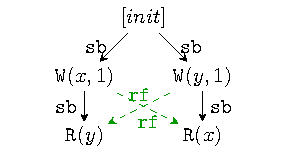
\includegraphics[scale=1.3]{figure/exec-graph/example.pdf} 
	\caption{Execution graph example} 
	\label{graph-example} 
\end{figure}







\section{C/C++ Memory Model}
C/C++ provides additional concurrency primitives, including atomics, mutex, threads and fences, along with an extensive specification of its memory model.
The first C/C++ memory model was described in a proposal\cite{c++model-proposal} in 2008, which was refined and formalized by \cite{c++model}. The following contents use the notations and definitions in \cite{c++model}, unless otherwise specified.

The memory model can be defined as a function, taking a set of candidate executions $X$ as input. These executions must be allowed by the operational semantics and are consistent, denoted as pre-executions. The function returns "NONE" if any executions have undefined behaviors; otherwise, it returns "SOME" pre-executions.

A candidate execution X contains two components, $X = (X_{opsem}, X_{witness})$, where $X_{opsem}$ is determined by the operational semantics and $X_{witness}$ is an existential witness of some further data. Both components are composed of memory actions (or actions for short) and relations. An action can be a non-atomic read or write, atomic operations, mutex operations and fences, represented by <aid, tid, type, location, value>. The $X_{opsem}$ contains three types of relations:

\begin{itemize}
	\item \textit{sequenced-before} (sb): A relation between intra-thread actions given by C/C++ language specifications, usually analogous to program order. When two separate actions are written in two separate statements, the former is sequenced before the latter. Arguments of functions or operands of some operators like '==' do not have specified evaluation order, thus do not have sequenced-before relations.
	\item \textit{additional-synchronized-with} (asw): The thread-creation action introduces an asw relation from the sequenced-before-maximal actions of the parent thread to the sequenced-before-minimal actions of the child thread.
	\item \textit{data-dependency} (dd):  The dd is provided by the operational semantics, primarily used for release/consume atomics. For example, a store to a pointer and the use of the pointed data have a dd relation.
\end{itemize}

In the SB example,  assuming that x and y are atomic variables, the $X_{opsem}$ of a candidate execution can be drawn as in Figure~\ref{XopsemSB}.
%   x = 0
%     | sb
%   y = 0
%   /asw    \asw
% x = 1     y = 1
%   |sb       |sb
% read y    read x

\begin{figure}[h!tbp] % htbp 表示优先放置位置:here, top, bottom, page
	\centering
	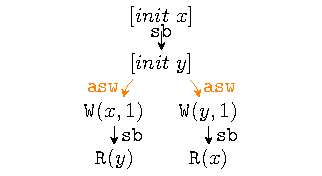
\includegraphics[scale=1.3]{figure/exec-graph/SB1.pdf} % 图片文件名和路径  
	\caption{$X_{opsem}$ of SB} % 图片标题
	\label{XopsemSB} % 图片标签,用于交叉引用
\end{figure}

The $X_{witness}$ part contains three additional relations. These relations are not uniquely determined by the operational semantics. Therefore, given a program p, the candidate execution X can have only one $X_{opsem}$, but multiple possible $X_{witness}$ configurations.

% $\wlab{1}{x, 0}$


\begin{itemize}
	\item \textit{read-from} (rf): An rf edge is established from a write action (non-atomic write, atomic write, or read-modify-write) to a read action (non-atomic read, atomic read, or read-modify-write) if the read action retrieves a value from the write action. Additionally, an rf edge is established between a lock action and its immediately preceding unlock action for the same mutex. The rf reads-from map is a function that includes all these rf relations in the execution.
	\item \textit{modification-order} (mo): This represents a total order of all writes to the same atomic location. Each location can have its own independent mo "chain," which is unrelated to chains for other locations.
	\item \textit{sequentially-consistent} (sc): This totally orders all mutex actions and actions with \texttt{mo\_seq\_cst} memory order.
\end{itemize}


In the SB example, assuming the initializations are non-atomic and other writes and reads are \texttt{mo\_seq\_cst}, a possible $X_{witness}$ for the SB example can be shown in Figure~\ref{XwitnessSB}
% rf
% x=1 -rf-> read x in thread2
% y=1 -rf-> read y in thread1
% sc
% x=1 -sc-> y=1 -sc-> read y -sc-> read x
% mo
% y=0 -mo-> y=1
% x=0 -mo-> x=1

\begin{figure}[htbp] % htbp 表示优先放置位置:here, top, bottom, page
	\centering
	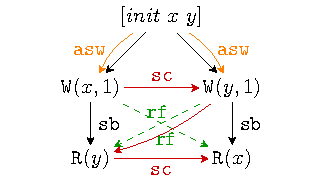
\includegraphics[scale=1.3]{figure/exec-graph/SB2.pdf} % 图片文件名和路径  
	\caption{$X_{witness}$ of SB} % 图片标题
	\label{XwitnessSB} % 图片标签,用于交叉引用
\end{figure}

There are some derived relations defined based on the above six relations. These derived relations will help to define the memory model and rule out illegal executions.

\begin{itemize}
	\item \textit{synchronizes-with} (sw): Every unlock action of a mutex has an sw edge pointing to the lock ordered after it in the sc order mentioned above. All asw relations are also sw relations. A read-acquire (read with \texttt{memory\_order\_acquire}) reading from a write-release gives rise to a sw relation. More generally, when the read-acquire R reads from a write W, it also synchronizes-with other write-release that is ordered before W in the modification order. However, not all write-releases preceding W can have sw relations with W, only those contained by the \textit{release sequence} of W. The definition of \textit{release sequence} is omitted here.
	\item \textit{happens-before} (hb): If the execution has no consume operations, the hb relation is a transitive closure of $sb \cup sw$. More generally, hb is defined as the union of sb and \textit{inter-thread-happens-before}, which includes the sw relation.
\end{itemize}


The three relations in $X_{witness}$ (rf, mo and sc) cannot be arbitrarily composed to make an execution. Instead, they have to satisfy some constraints, called \textit{coherence}. The coherence constraints have the form "A-B Coherence", or CoAB, where both A and B are either reads or writes, and $A \xrightarrow{\text{hb}} B$. As illustrated previously, the hb is derived from sb and sw, where sw is derived from sc and rf. The constraints on hb, mo and rf will ultimately constrain the combinations of rf, mo and sc. The coherence constraints are listed below:

\begin{itemize}
	\item \textit{Read-Read Coherence} (CoRR): Two reads ordered by hb cannot read from two writes ordered by mo in the other direction.
	\item \textit{Write-Read Coherence} (CoWR): When a write, $w$, happens before a read $r$, $r$ cannot read from a write that precedes $w$ in mo.
	\item \textit{Write-Write Coherence} (CoWW): The mo and hb relations of two writes, $w_1$ and $w_2$, should have same directions. For instance, $w_1 \xrightarrow{\text{mo}} w_2 \land w_2 \xrightarrow{\text{hb}} w_1$ is not allowed.
	\item \textit{Read-Write Coherence} (CoRW): When a read happens before a write $w$, it cannot read from a write that is ordered after $w$ in mo. This forbids the $rf \cup hb \cup mo$ to be cyclic.
\end{itemize}



Consider the SB example. If the reads and writes are SC atomic operations, the execution shown in Figure~\ref{NotAllowedSB}, where both reads read the value 0, is not allowed because this execution violates the CoWR constraint. However, if the reads and writes are relaxed, then both reads reading the value 0 from the initializations is permitted.


\begin{figure}[htbp] % htbp 表示优先放置位置:here, top, bottom, page
	\centering
	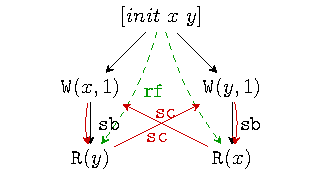
\includegraphics[scale=1.3]{figure/exec-graph/SB3.pdf} % 图片文件名和路径  
	\caption{Not-allowed of SB} % 图片标题
	\label{NotAllowedSB} % 图片标签,用于交叉引用
\end{figure}
% rf
% x=0 -rf-> read x in thread2
% y=0 -rf-> read y in thread1
% sc
% x=1 -sc-> y=1 -sc-> read y -sc-> read x
% mo
% y=0 -mo-> y=1
% x=0 -mo-> x=1
% \begin{figure}
  %\footnotesize
  \centering
  \begin{tikzpicture}[yscale=0.85]
    \node (s) at (0,0)  {\begin{tabular}{c}$i: [X=Y=0]$ \\ {\footnotesize\color{teal}$\set{(X,i_x),(Y,i_y)}$}\end{tabular}};
    \node (t11) at (-3,-2)  {\begin{tabular}{c}$e_1: \W(X,1)$ \\ {\footnotesize\color{teal}$\set{(X,e_1),(Y,i_y)}$}\end{tabular}}; 
    \node (t21) at (0,-2)  {\begin{tabular}{c}$e_2: \R(X, 1)$  \\ {\footnotesize\color{teal}$\set{(X,e_1),(Y,i_y)}$}\end{tabular}};
    \node (t22) at (0,-4) {\begin{tabular}{c}$e_3: \W(Y,1)$ \\ {\footnotesize\color{teal}$\set{(X,e_1),(Y,e_3)}$}\end{tabular}};
    \node (t31) at (3, -2)  {\begin{tabular}{c}$e_4: \R(Y, 1)$ \\ {\footnotesize\color{teal}$\set{(X,i_x),(Y,e_3)}$}\end{tabular}};
    \node (t32) at (3, -4) {\begin{tabular}{c}$e_5: \R(X, 0)$ \\ {\footnotesize\color{teal}$\set{(X,i_x),(Y,e_3)}$}\end{tabular}};
  
  % \node at (1.2,-1.75)  {{\footnotesize\color{blue}$\set{(X,e_1)}$}};
  % \node at (3.7,-1.75)  {{\footnotesize\color{blue}$\set{(Y,e_3)}$}};
  
  %
    \draw[po] (s) to node[right]{(1)} (t11);
    \draw[po] (s) to node[right]{(2)} (t21) ;
    \draw[po] (t21) to node[right]{(3)} (t22);
    \draw[po] (s) to node[right]{(4)} (t31);
    \draw[po] (t31) to node[right]{(5)} (t32);
    \draw[rf] (t11) to node[above]{(2)} node[below]{$\rf$} (t21) ;
    \draw[rf] (t22) to node[above]{(4)} node[below]{$\rf$} (t31) ;
  \end{tikzpicture}
  %\caption{A $d=2$ execution of Program~\ref{prg:MP2} that hits the assertion violation}
  \caption{A $d=2, \; h=1$ execution of MP2. The illustrated execution selects $[e_2, e_4]$ as the sinks of the two communication relations and assigns initial priorities as $[T1, T2, T3]$.}
  \label{fig:mp2:d2}
  \end{figure}



The C/C++ memory model described above is an axiomatic model that specifies which executions are allowed and which are not. However, this model has some flaws. Firstly, the data-dependency relation and those associated with consume-release atomics are specified but are not implemented on most platforms, where they are typically treated as acquire-release atomic operations. Furthermore, there are some executions that are allowed by the model but should be ruled out in principle. For instance, consider a load buffer (LB) program where two threads load from different locations and store the loaded values to the other location. If all the atomic operations have a relaxed memory order, any loaded value is allowed by the model. This issue is known as the \textit{out-of-thin-air} (OOTA) problem. Since the model was proposed, numerous efforts have been made to revise it, which will be summarized in Section~\ref{cha:related}.


